\documentclass[a4paper,12pt]{article}
\setlength{\hoffset}{-0.2cm}
\setlength{\voffset}{-2cm}
\setlength{\textheight}{25cm} 
\setlength{\textwidth}{14cm}
\renewcommand{\figurename}{Obr.č.}
\usepackage{graphicx}
\author{Marek Polčák}

\begin{document}
\title{Robotické protézy ruky}
\maketitle

\section*{Úvod}

Tato práce se věnuje problematice robotických protéz rukou, které zaznamenávají v poslední době rozmachu elektroniky výrazný posun, jelikož je možné zmenšovat elektronické součástky, tak je možné protézy odlehčovat. Dle statistiky Evropské komise se ročně stane v Evropské Unii 12000 pracovních úrazů, které končí traumatickou amputací. Dlouhou dobu se vývoj protéz neposouval a protézy byly jednak nepříliš estetické a ne tolik efektivní.\cite{Euro}\par
 
Hlavní problematikou je samotné ovládání ruky, jelikož postižený člověk nedokáže přímo ruku ovládat nervovou soustavou. Protézy existují v různých formách, jelikož se jejich konstrukce odvíjí od velikosti postižení. Tato práce se věnuje především protézám předloktí a ruky.

\section{Krátká historie protéz rukou}

První funkční náhrada a ruky, která nesloužila pouze pro její kosmetické účely, byla navržena již v 16. století lékařem Ambroisem Paré, který sloužil několik anglickým králům. Z tohoto období se dochoval i funkční exemplář protézy, která již měla v sobě uložený mechanismus umožňující aretaci prstů v několika pozicích. Palec byl ovládán separátně a společně s prsty musely být manuálně zaaretovány. Tato ruka vážila 1.6 kg, což je poměrně hodně, jelikož ruka sloužila jako návlek. Již zde však mohl postižený držet v ruce zaaretovaný předmět a využívat tak zdravou ruku k jiným činnostem.\cite{Chappell}

 
\begin{figure}[b!]
\centering
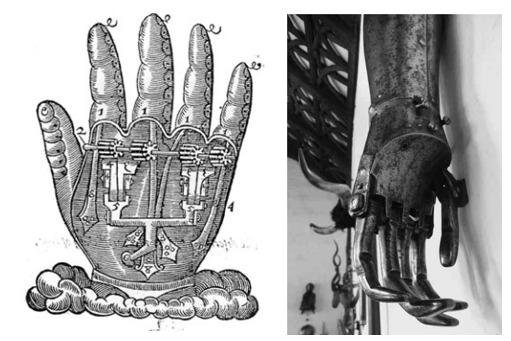
\includegraphics[scale=0.6]{figures/Historic_hand_prosthesis.PNG}
\caption{Nejstarší dochovaná mechanická protéza ruky \cite{Chappell}}
\end{figure}\break
V průběhu času se objevovaly koncepty více méně obdobné, nebo dokonce jednodušší. V průběhu 19. století se vyvinula protéza poháněná tělem, což spočívalo ve využití síly svalového kloubu, který při stažení ruku otevřel. Tyto protézy využívaly pouze dvou protichůdných prstů, takže se těžko dala protéza kosmeticky upravit. Výhodou byla nízká cena a jednoduchost.\cite{Fukushima}

Ve 20. století byly vyvinuty myoelektrickcé protézy, které se vyznačoval tím, že zdravé svaly ruky vyvolaly elektrický impulz, který byl zaznamenán elektrodami umístěných na svale. Tento signál byl řídícím signálem pro otevření či uzavření ruky. Tyto protézy měly tu výhodu, že bylo možné využít již silnější avšak kompaktní aktuátory, které se daly dále zpřevodovat. Nevýhodou byla latence systému, která pramenila především v nedokonalé podobě elektrod.\cite{Fukushima}\par

\section{Konstrukce protéz ruky}
Jelikož je cílem, se přibližovat vysoké citlivosti a přesnosti lidské ruky, tak se snaží vědci a výzkumníci posouvat kinematiku ruky co nejblíže zdravé ruce. Lidská ruka je neuvěřitelné složitý mechanismus, takže se bohužel se nedá očekávat, že se protézy do takové úrovně dostanou. Aktivní protézy využívají buď zpřevodovaného mechanismu nebo lanka. Obě konstrukce mají své výhody a nevýhody.\cite{Chappell}\par

Robotická protéza je složena z aktivní části a řídící části, jak je tomu u většiny robotických zařízení. Pod aktivní částí si lze představit elektrické aktuátory, baterii a mechanismus distribuující energii do jednotlivých článků prstů. Řídící část je přímo navázána na jak část aktivní, tak část senzorů. Na tuto část protéz je v poslední době kladen zvláštní důraz, jelikož se snaží jednak zrychlovat odezvu, tak zlepšovat propojení mezi nervovou soustavou člověka a protézy a to například propojením zpětnou vazbou, což již vytváří z protézy regulační obvod. Následující obrázek prezentuje obecné schéma protézy.\cite{Chappell}


\begin{figure}[b!]
\centering
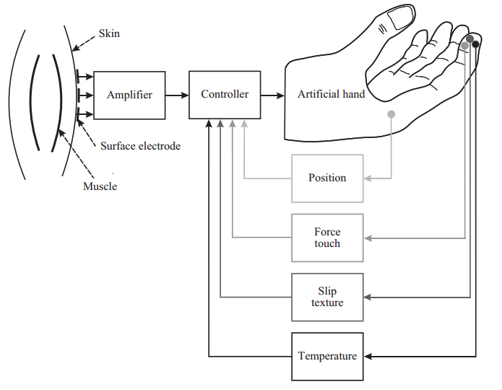
\includegraphics[scale=0.8]{figures/Rizeni_roboticke_protezy.PNG}
\caption{Schematický popis systému robotické protézy ruky \cite{Chappell}}
\end{figure}\break

Hmotnost je u protéz nepřítel, jelikož je cílem přiblížit hmotnost protézy zdravé ruce, ba dokonce snížit její hmotnost. Lidská ruka má 22 stupňů volnosti a váží asi 400 g, čemuž bude problematické se někdy přiblížit jelikož hmotnost baterie zůstane dosti velká. Toho se ovšem dosahuje poměrně těžce, jak ukazuje i následující graf, který ukazuje hmotnostní rozložení jednotlivých komponent ruční protézy. Z grafu je patrné, že největší hmotnostní podíl tvoří aktuátory a mechanismy, z nichž už se horko těžko snižuje hmotnost.\cite{Chappell}\cite{Jung}

\begin{figure}[hbtp]
\centering
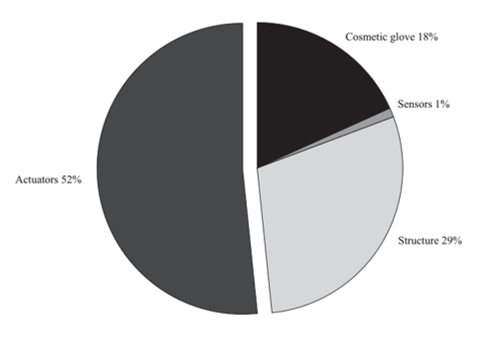
\includegraphics[scale=0.8]{figures/Hmotnosti_casti_protezy.PNG}
\caption{Hmotnostní rozložení komponent robotické protézy ruky \cite{Chappell}}
\end{figure}

\subsection{Konstrukční provedení protézy s ozubením}
Nejjednoduššími protézami jsou bezesporu protézy s ozubením a jde již spíše o historický mechanismus v tomto odvětví. Pomocí ozubených kol lze přenést kroutící moment pouze na prst jako takový a prsty tak fungují spíše jako kleště, jelikož klouby jednotlivých článků mají 0 stupňů volnosti. Každý prst má jako celkem 1 stupeň volnosti. Další problém je také ovládání prstů separátně, což vyžaduje pokročilejší mechanismus.\cite{Chappell}
\pagebreak 

\begin{figure}[t!]
\centering
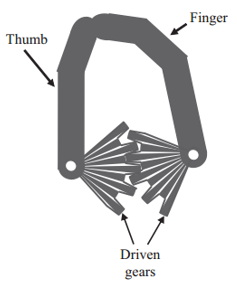
\includegraphics[scale=0.9]{figures/Clamp_fingers.PNG}
\caption{Jednoduchá klešťovitá protéza s ozubením \cite{Chappell}}
\end{figure}

\subsection{Konstrukční provedení s integrovanými aktuátory}
Několik konceptů zabudovává malé motory do článků prstu a převedení pohybu na další články se provádí pomocí drátů napojených šnekové soukolí, které je napojeno na motor. Toto konstrukční provedení umožňuje již protéze provádění složitějších úchopů a gest. Tento koncept by měl být oproti komerčně dostupným řešením lepší v tom, že klouby dokáží vyvinout vyšší úhlovou rychlost a lze s ním dosáhnout srovnatelných úchopů jako u ostatních konceptů. Robotická protéza dokáže vyvinout maximální stisk 120 N, ale běžně kolem 40 N. Využívá baterie má kapacitu 2000 mAh a napětí 7.4 V.\cite{Jung}

\begin{figure}[hbp]
\centering
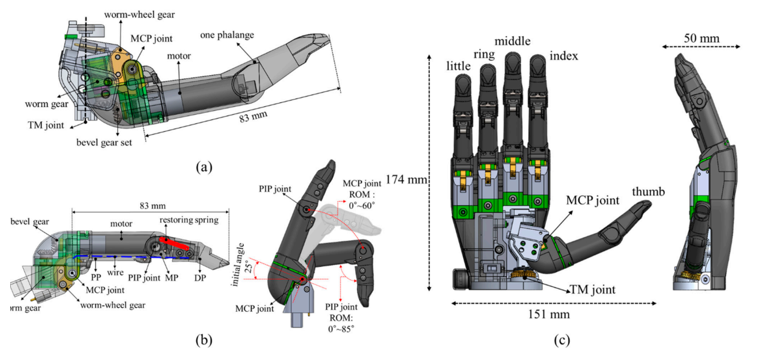
\includegraphics[scale=0.7]{figures/Infinger_actuator_schematics.PNG}
\caption{Robotická protéza s integrovanými aktuátory \cite{Jung}}
\end{figure}\break

\subsection{Konstrukční provedení lankové protézy}
Lankové protézy poháněné elektrickými motory využívají kladkové mechanismy, které ovládají několik prstů zároveň - ukazováček, prostředníček, prsteník a malíček. Jde o poměrně komplikovaný mechanismus, který je založen mechanismu ruky TUAT/Karlsruhe. V jednotlivých kloubech jsou poté další kladky, takže se ruka při sevření chová podobně jako zdravá ruka. Palec má zpravidla separátní aktuátor a jeden stupeň volnosti. Tento koncept funguje dobře pro uchopování předmětů různých tvarů, přestože se aktivuje několik prstů zároveň. Nevyužité prsty zůstávají sevřeny. Pokud je jeden prst zablokovaný předmětem, lanko se namotává kolem kladky umožňující dále prst svírat, který ještě není zablokovaný. Bohužel tedy nelze tento koncept využít na úlohy jemné motoriky. Ruka KIT využívá 12 V baterie na pohon kontroléru i motorů. Lankové protézy většinou dosahují menších úchopů, okolo 24 N (KIT), což je limitováno jednak aktuátory a poté pevností lanek.\cite{KIT}
\begin{figure}[hbtp]
\centering
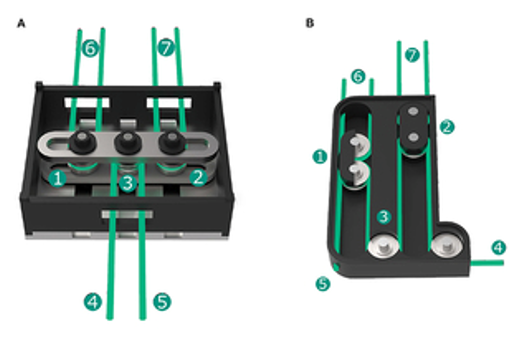
\includegraphics[scale=0.85]{figures/KIT_string_hand.PNG}
\caption{Robotická protéza ruky s lankovým převodem \cite{KIT}}
\end{figure}

\subsection{Materiály}
Tím, že mají protézy sloužit lidem v každodenním životě, je potřeba, aby byla jejich váha co nejnižší a zároveň protéza vykazovala dostatečnou pevnost a životnost. Z toho důvodu se u dražších protéz využívá duralových slitin či dokonce hořčíkových slitin u více namáhaných součástí. Povrch ruky se snaží často kůži silikonovým provedením nebo zůstává nekryt a je vidět ať už kompozitní nebo platové jádro prstů. V poslední době se hojně využívá 3D tisku a open-source komunita napomáhá tomu, aby si člověk mohl takovou ruku alespoň pro výzkum vytisknout sám.\cite{Chappell}\cite{3DPRINT}
\pagebreak

\subsection{Sensory}
\subsubsection{EMG sensory}
Elektromyografické (EMG) sensory jsou sensory zachycující změnu elektrického potenciálu, který vzniká depolarizací svalových vláken při jejich kontrakci a relaxaci. Využívají se mimo jiné i pro monitoring zdravotního stavu. Výhodou je, že je lze aplikovat povrchově. Stačí je přilepit na povrch kůže. Přesnost senzorů závisí také na kvalitě povrchového EMG na vlastnostech pokožky (např. suchost, čistota, mastnota) nebo relativní pohyb mezi elektrody a svalová vlákna.\cite{Jung}\cite{EMGs}

\begin{figure}[hbtp]
\centering
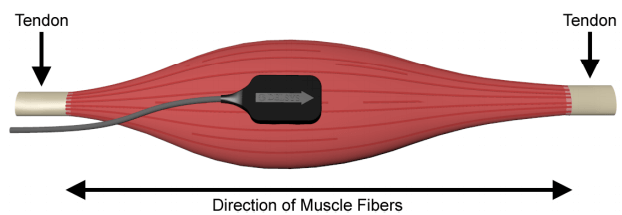
\includegraphics[scale=0.6]{figures/emg-sensor-placement-1.png}
\caption{Správná orientace EMG sensoru \cite{EMGs}}
\end{figure}

\subsubsection{FSR sensory}
Existuje i jiná metoda, která nezaznamenává elektrické impulzy, ale síly a tlaky. Těmito sensory jsou force-sensitive resistors (FSR). FSR se skládají z vodivého polymeru, mění svůj odpor při působení síly. Funguje dobře i v mírně nepřátelském prostředí a není tolik závislý na správném ošetření povrchu kůže. Jejich cena je poměrně nízká.\cite{Jung}

\begin{figure}[hbtp]
\centering
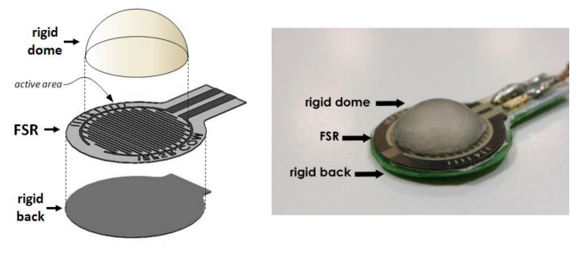
\includegraphics[scale=0.9]{figures/FSR_sensor.PNG}
\caption{Konstrukce FSR sensoru \cite{Jung}}
\end{figure}\break


\subsection{Řízení robotické protézy}
Dlouhou dobu byly myoelektrické protézy založeny na přímém řízení člověkem, který se musel soustředit na každý pohyb ruky, jelikož musel zapojit správné svaly zdravé části těla, aby došlo k přečtení signály zpravidla EMG sensory. To je pro člověka nesmírně zatěžující a únavné, pokud se musí soustředit na každý úchop. Pro lidi, kterým byla amputována celá lze využít cílové svalové reinvervace, kdy jsou nervy ruky chirurgicky napojeny na prsní svaly, na které jsou poté umístěny EMG sensory a člověk i tak dokáže ovládat protézu.
Nejideálnější varianta řízení by bylo napojení robotické protézy na nervový systém člověka, což je bohužel zatím ve stádiu výzkumu.\cite{Chappell}\cite{Tongue}

\subsubsection{Řízení protézy pomocí pohybem jazyka}
Jeden koncept využívá k ovládání protézy ITCS – Inductive Tongue Control System, který využívá pohybu jazyka, což s sebou přináší jisté výhody pro pacienty s těžkým postižením. ITCS se skládá z ústní části a centrální jednotky. Každá ústní část je přizpůsobena uživateli a vyrobena dle zubního otisku oblasti horního patra zhotovený zubním lékařem. Ústní část se skládá ze dvou desek plošných spojů s celkem 18 senzory a obvody bezdrátového nabíjení (cívka a baterie), elektronické obvody potřebné pro předběžné zpracování signálu a bezdrátovou komunikaci.\cite{Tongue}
\\
Na špičku jazyka je přilepen aktivátor sensorů, kterým se poté člověk dotýká jednotlivých částí horního patra dutiny ústní, po které jsou rozděleny sensory pro jednotlivé pohyby ruky. Systém v článku využíval kabelové napojení, uložené v silikonové trubičce, na vysílací jednotku připevněnou na hrudi člověka.\cite{Tongue}

\begin{figure}[hbtp]
\centering
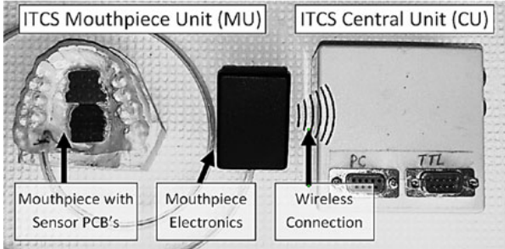
\includegraphics[scale=1]{figures/ITCS_control.PNG}
\caption{ITCS systém \cite{Tongue}}
\end{figure}\break

\subsubsection{Semi-autonomní robotická protéza}
V poslední době se již vyvíjí polo-autonomní protézy, jako např. projekt KIT, kdy se využívá přídavné polohové sensory polohy motorů a RGB kameru, která je integrovaná v dlani ruky. Projekt KIT se spoléhá na metody strojového vidění. Rozpoznaný obraz je poté zpracován interovaným systémem využitím konvolučních neuronových sítí, které na základě databáze předmětů dokáží rozpoznat předmět a poté vyvinou adekvátní sílu úchopu na základě hodnot databáze. Ruka KIT má také integrovaný Bluetooth, který integruje data z proprioceptivních sensorů, obraz a zpětnou vazbu od uživatele.\cite{KIT}

\begin{figure}[hbtp]
\centering
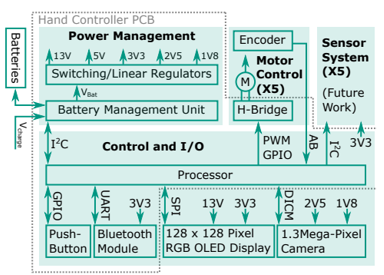
\includegraphics[scale=1]{figures/Camera_hand.PNG}
\caption{Řízení robotické protézy ruky KIT \cite{KIT}}
\end{figure}

\subsubsection{Haptická odezva}
Člověk využívající protézu ruky nedokáže bez jednoznačné odezvy odhadnout, jakou silou uchopit předmět, aniž by ho nepoškodil, jelikož doposud nebylo možné přenést hmatovou odezvu. Několik vědeckých týmu se věnuje této problematice a bylo již možné zaznamenat první funkční prototypy. Některé protézy využívají haptickou odezvu jiných zdravých částí těla, např. prstů nohou, kdy se robotická protéza ruky ovládá palcem nohy a speciální mechanismus vytváří adekvátní odezvu odpovídající stisku robotické ruky. Člověk tak dokáže dosáhnou většího citu při uchopování křehkých předmětů.\cite{Fukushima}\par
Efektivnější a pro člověka realističtější možnost je napojení elektrod na zdravé nervy ruky, které byly napojeny na nervy prstů. Robotická s haptickou odezvou zpracuje data o dotyku a vyšle je elektrodám.\cite{Haptic}
\pagebreak

\section{Závěr}
Robotické protézy ruky zaznamenávají v poslední době velký pokrok a mnoho lidí se již za protézy nemusí stydět, jelikož v době kultovních komiksových a cyberpunkových subkultur jsou jakékoli úpravy lidského těla již nenarušují konsenzus společnosti. K tomu, aby se robotické protézy přiblížily schopnostem lidské ruky, by bylo zapotřebí napojit řízení robotické protézy  na nervovou soustavu, čehož se snad v blízké době dočkáme. Další vývoj by se mohl zaměřit také na optimalizaci aktuátorů, aby byly lehčí a menší, což by pomohlo spíše pro aplikace jemné motoriky než dosahování maximálních stisků.
\pagebreak
\begin{thebibliography}{1}
  \bibitem[1]{Chappell} CHAPPELL  Paul H.:
    \emph{Mechatronic hands: Prosthetic and Robotic design}. Institution of Engineering and Technology,
    London, 2016. ISBN 978-1-78561-155-1.
  \bibitem[2]{Euro} European Comission, Eurostat:
    \emph{Accidents at work by NACE Rev. 2 activity and type of injury}. (Luxembourg, 2017).\\
    \verb|http://appsso.eurostat.ec.europa.eu/nui/show.do?dataset=hsw n2 07& lang=en|
    
  \bibitem[3]{Fukushima} FUKUSHIMA, Satoshi, Takahiro NOZAKI a Kouhei OHNISHI:
    \emph{Development of haptic prosthetic hand for realization of intuitive operation}. IECON 2016 - 42nd Annual Conference of the IEEE Industrial Electronics Society,
    IEEE, 2016. ISBN 978-1-5090-3474-1.
    
  \bibitem[4]{Jung} JUNG, Sung-Yoon, Seung-Gi KIM, Joo-Hyung KIM a Se-Hoon PARK:
    \emph{Development of Multifunctional Myoelectric Hand Prosthesis System with Easy and Effective Mode Change Control Method Based on the Thumb Position and State}. Applied Sciences. 2021,ISSN 2076-3417.  
    
    \bibitem[5]{Fukaya} FUKAYA, N., S. TOYAMA, T. ASFOUR a R. DILLMANN:
    \emph{Design of the TUAT/Karlsruhe humanoid hand}. International Conference on Intelligent Robots and Systems.  IEEE, 2000,,ISBN 0-7803-6348-5. 
    
    \bibitem[6]{KIT} WEINER, Pascal, Julia STARKE, Felix HUNDHAUSEN, Jonas BEIL a Tamim ASFOUR:
    \emph{The KIT Prosthetic Hand: Design and Control}. International Conference on Intelligent Robots and Systems.  IEEE, 2018,,ISBN 978-1-5386-8094-0.
    
     \bibitem[7]{3DPRINT} SULLIVAN, Mark; OH, Bryan; and TAYLOR , Ian:
    \emph{3d Printed Prosthetic Hand}. Mechanical Engineering 
Design Project Class. 65.  2017,https:/ /openscholarship.wustl.edu/mems411/65 
    
     \bibitem[8]{EMGs} SHAWN:
    \emph{What is EMG sensor, Myoware and How to use with Arduino?}. Seeedstudio [online]. 2020 [cit. 2022-04-10],https://www.seeedstudio.com/blog/2019/12/29/what-is-emg-sensor-myoware-and-how-to-use-with-arduino/

	\bibitem[9]{Tongue} JOHANSEN, Daniel, Christian CIPRIANI, Dejan B. POPOVIC a Lotte N. S. A. STRUIJK:
    	\emph{Control of a Robotic Hand Using a Tongue Control System—A Prosthesis Application}.IEEE Transactions on Biomedical Engineering. 2016,ISSN 0018-9294arduino/
    	
    \bibitem[8]{EMGs} SHAWN:
    	\emph{What is EMG sensor, Myoware and How to use with Arduino?}. Seeedstudio [online]. 2020 [cit. 2022-04-10],https://www.seeedstudio.com/blog/2019/12/29/what-is-emg-sensor-myoware-and-how-to-use-with-arduino/
    	
    \bibitem[9]{Haptic} TYLER, Dustin J.:
    	\emph{Creating a Prosthetic Hand That Can Feel.}. IEEE Spectrum [online]. 28 APR 2016 [cit. 2022-04-10],https://spectrum.ieee.org/creating-a-prosthetic-hand-that-can-feel
    
    
\end{thebibliography}

\end{document}
